\documentclass[12pt, aspectratio=169]{beamer}
\usetheme{Madrid}
\usecolortheme{seahorse}
\usepackage{graphicx}
\usepackage{amsmath}
\usepackage{bookmark}
\usepackage{booktabs}
\usepackage[most]{tcolorbox}
\usepackage{xcolor}
\usepackage{caption}
\captionsetup[table]{justification=raggedright, singlelinecheck=false}
\definecolor{theme}{RGB}{214, 214, 240}

\graphicspath{{images/}} 


\title[Forecasting Refined Sugar Prices]{\uppercase{Forecasting the Price of Refined Sugar in the Philippines Using ARIMAX Model}}
\author{Alanan, Baldeo, Hilario, Rivera, Santos}
\institute{Bulacan State University \\ BS Mathematics with Specialization in Computer Science}
\date{May 2025}

\begin{document}

% Title Slide
\begin{frame}
  \titlepage
\end{frame}

% Introduction
\begin{frame}{Introduction}
Sugar plays a vital role in the Philippine economy, serving as a key ingredient in household consumption and food manufacturing, while also supporting over 1.5 million jobs and contributing 2\% to the national GDP. Most sugarcane is produced in Negros Occidental, the country's “Sugar Bowl.” However, the industry faces challenges including climate disruptions, declining productivity, and rising demand. These factors, along with typhoons and international price volatility, have led to production shortfalls and increased reliance on imports. As refined sugar prices continue to rise, this study aims to forecast future price movements using mathematical modeling that incorporates external factors to inform decisions in agriculture, industry, and policy-making.
\end{frame}

% Statement of the Problem

\begin{frame}{Statement of the Problem}
    The price of refined sugar is influenced by various factors such as climate conditions, sugar production, government policies, and global market trends. Changes in sugar prices have a direct impact on Filipino households, food manufacturers, and businesses that rely on sugar as a primary ingredient. Despite its economic and social significance, there is limited research on accurately forecasting sugar prices using mathematical models that incorporate both historical price data and external variables to forecast future price movements.
\end{frame}

\begin{frame}{Statement of the Problem}
This study aims to develop a forecasting model for the prices of refined sugar in the Philippines using the AutoRegressive Integrated Moving Average with Exogenous Variables (ARIMAX) model. The model integrates external factors such as production and withdrawals of refined sugar, global sugar prices, exchange rate from USD to PHP, temperature, total precipitation, and inflation to improve the reliability of forecast.
\vspace{12pt}

    This study seeks to answer:
    \begin{enumerate}
        \item Which external factors influence sugar prices and how strongly?
        \item Can ARIMAX provide accurate forecasts?
        \item What are the projected sugar prices for early 2025 and through 2027?
    \end{enumerate}

\end{frame}


% Objectives
\begin{frame}{Research Objectives}
  \begin{itemize}
    \item Identify external factors influencing refined sugar prices.
    \item Evaluate ARIMAX model for forecasting accuracy.
    \item Forecast short- and long-term prices up to 2027.
  \end{itemize}
\end{frame}

\begin{frame}
\frametitle{Scope and Delimitations}

    \begin{itemize}
        \item Monthly refined sugar prices in the Philippines from 2014 to 2024.
        \item Uses ARIMAX model with exogenous variables: climate (Negros Region), sugar production, global prices, exchange rate, inflation, and withdrawals.
        \item Focus is only on refined sugar; excludes washed, brown sugar, and molasses.
        \item Climate data limited to Negros Region, the largest sugar-producing area.
        \item Import data excluded due to inconsistent monthly availability; withdrawals used to proxy demand.
        \item Does not cover sugar-based product prices (e.g., pastries, beverages).
    \end{itemize}
\end{frame}


%Prelims
\begin{frame}
\frametitle{Preliminaries}
This section introduces key concepts used in the modeling process of forecasting, particularly relevant to time series analysis.
\begin{itemize}
    \item Time Series Analysis
    \item ARIMAX Model
    \item Stationarity (ADF Test)
    \item ACF and PACF
    \item Ljung-Box Test
    \item VIF
    \item AIC and BIC
\end{itemize}
\end{frame}

\begin{frame}
\frametitle{Time Series Analysis}
\begin{itemize}
    \item A time series is a sequence of data points recorded at uniform time intervals.
    \item Analysis involves identifying patterns like trends and seasonality, and forecasting.
    \item Denoted as $\{y_t\}$, where each $y_t$ is associated with time $t$.
    \item Observations are usually ordered chronologically.
\end{itemize}
\end{frame}

\begin{frame}
\frametitle{ARIMAX Model}
\begin{itemize}
    \item Extension of ARIMA that incorporates exogenous variables.
    \item Requires the time series to be \textbf{stationary} (constant mean and variance).
    \item ARIMA combines:
    \begin{itemize}
        \item \textbf{AR} (AutoRegressive): The value of the current observation is affected by the previous observations.
        \item \textbf{I} (Integrated): Differencing to achieve stationarity
        \item \textbf{MA} (Moving Average):It captures the errors from previous observations and how it affects the current observation.
    \end{itemize}
    \item ARIMAX includes external factors to enhance forecasting.
\end{itemize}
\end{frame}

\begin{frame}
\frametitle{ADF Test for Stationarity}
\begin{itemize}
    \item Tests if a time series has a unit root (non-stationary).
    \item Null Hypothesis $H_0$: Series has a unit root.
    \item If p-value $<$ 0.05, reject $H_0$ $\Rightarrow$ series is stationary.
    \item Differencing can be applied to make non-stationary series stationary.
\end{itemize}

\end{frame}

\begin{frame}
\frametitle{ACF and PACF}
\begin{itemize}
    \item \textbf{Autocorrelation Function}:\\ Correlation between series and its lagged values.
    \item \textbf{Partial Autocorrelation Function}:\\ Correlation with lagged values removing shorter lags.
    \item \textbf{Interpretation Tips:}
    \begin{itemize}
        \item If ACF tails off and PACF cuts off → AR model.
        \item If PACF tails off and ACF cuts off → MA model.
        \item If both tail off gradually → consider ARMA or ARIMA.
    \end{itemize}
\end{itemize}
\end{frame}

\begin{frame}{Ljung-Box Statistics Test}
    Test whether residuals from a time series model exhibit autocorrelation (i.e., differ from white noise). 
    
    \vspace{0.2cm}
    \textbf{Hypotheses:}
    \begin{itemize}
        \item $H_0$: Residuals are independently distributed (white noise)
        \item $H_a$: Residuals are autocorrelated (model has lack of fit)
    \end{itemize}
    \textbf{Decision Rule:}
    \begin{itemize}
        \item If \textbf{p-value $>$ 0.05}: Fail to reject $H_0$ $\rightarrow$ residuals resemble \textbf{white noise}
        \item If \textbf{p-value $\leq$ 0.05}: Reject $H_0$ $\rightarrow$ residuals exhibit \textbf{autocorrelation}
    \end{itemize}
    
    \vspace{0.2cm}
    A model with white noise residuals is considered well-fitted for forecasting.
\end{frame}

\begin{frame}
\frametitle{Variance Inflation Factor (VIF)}
\begin{itemize}
    \item Detects multicollinearity among exogenous variables.
    \[
    VIF_i = \frac{1}{1 - R_i^2}
    \]
    \item $R_i^2$: Coefficient of determination for $i$-th variable regressed on others.
    \item VIF $>$ 5 (or 10): Potential multicollinearity issue.
\end{itemize}
\end{frame}

\begin{frame}{Model Selection: AIC and BIC}
    Compare multiple models to identify the best-fitting model with the right balance of fit and complexity.
    
    \vspace{0.3cm}
    \textbf{Akaike Information Criterion (AIC):}
    \begin{itemize}
        \item Measures goodness of fit while penalizing model complexity.
        \item Lower AIC → Better model.
    \end{itemize}

    \vspace{0.2cm}
    \textbf{Bayesian Information Criterion (BIC):}
    \begin{itemize}
        \item Similar to AIC, but imposes a stronger penalty for complexity.
        \item Tends to prefer simpler models compared to AIC.
    \end{itemize}
    
    \vspace{0.2cm}
    Both criteria aim to select models with good predictive performance, but \textbf{BIC penalizes complexity more heavily}.
\end{frame}




% Methodology
\begin{frame}
    \begin{tcolorbox}[colframe=theme, colback=theme]
        \begin{center}
            \Huge{Methodology}
        \end{center}
    \end{tcolorbox}
\end{frame}

\begin{frame}{Methodology}
    \begin{itemize}
        \item     This study will employ a quantitative research design using time series analysis to forecast the price of refined sugar in the Philippines.
        \item The main forecasting technique to be used is the Autoregressive Integrated Moving Average with Exogenous Variables (ARIMAX) model.
    \end{itemize}
\end{frame}

\begin{frame}{Datasets}
The dataset used in this study consists of monthly time series data from September 2014 to August 2024. 

\vspace{12pt} 

\textbf{Target variable:} Price of refined sugar in the Philippines\\

\textbf{Exogenous variables:}
\begin{itemize}
    \item Climate data (temperature, precipitation) in Negros Region. 
    \item Production and Withdrawals of refined sugar. 
    \item Global Price of sugar. 
    \item Exchange rate from PHP to USD. 
    \item Inflation rate. 
\end{itemize} 
\end{frame}

\begin{frame}{Procedures}
    \begin{block}{Analytical Procedure}
        The analytical procedure for the model development and validation is done in Python using various libraries such as \texttt{pandas, statsmodels, sklearn, pmdarima, matplotlib}.
    \end{block}
\end{frame}

% Data Preparation
\begin{frame}{Data Preparation}
    \begin{itemize}
        \item Making sure all of the data are aligned in monthly intervals and handling the missing data points. 
        \item The missing data points are filled using the \texttt{forward\_fill()} function from \texttt{pandas} library in Python.
        \item Split the dataset into training and testing sets
    \end{itemize}
\end{frame}

% Stationarity Test
\begin{frame}{Stationarity Test}
    \begin{itemize}
        \item The Augmented Dickey-Fuller (ADF) test is conducted on each variable to test for stationarity. 
        \item The \texttt{adfuller()} function from the \texttt{statsmodels} library in Python is used to perform the test.
        \item If the variable is not stationary (p-value $>$ 0.05), perform differencing to eliminate the presence of trend or seasonality.
        \item If it is still non-stationary, differentiate it again until it achieves stationarity.
    \end{itemize}
\end{frame}

% Model Identification
\begin{frame}{Model Identification}
    \begin{itemize}
        \item Finding the appropriate order of ARIMAX($p,d,q$) parameters through the plot of Autocorrelation Function (ACF) and Partial Autocorrelation Function (PACF).
        \item The AR components are determined using the PACF plot, where lags with significant spikes are the possible order for the AR component.
        \item The MA components are determined using the ACF plot, where lags with significant spikes are the possible order for the MA component.
        \item The Integrated $I$ component is determined based on the order of differencing required to achieve stationarity
    \end{itemize}
\end{frame}

% Model Estimation and Selection
\begin{frame}{Model Estimation and Selection}
    \begin{itemize}
        \item All possible ARIMAX models are fitted using the training set and evaluated for accuracy with the test set.
        \item Each model is assessed based on mean absolute percentage error (MAPE) to measure forecasting accuracy. 
        \item Akaike Information Criterion (AIC) and Bayesian Information Criterion (BIC) are used to penalize model complexity.
        \item The best ARIMAX model is selected based on the lowest values of AIC, BIC, and MAPE.
    \end{itemize}
\end{frame}

% Model Diagnostics and Interpretation
\begin{frame}{Model Diagnostics and Interpretation}
    \begin{itemize}
        \item The residuals of the selected model are examined using the Ljung-Box test to ensure that the residuals resemble white noise.
        \item The coefficients of the variables are interpreted based on their significance (p-values).
        \item Variance Inflation Factor (VIF) may be calculated to assess multicollinearity among exogenous variables
    \end{itemize}
\end{frame}


% Forecasting
\begin{frame}{Forecasting}
    \begin{itemize}
        \item Once the best-performing ARIMAX model is selected, it is used to forecast the monthly retail price of refined sugar in the Philippines.
        \item For forecasting each exogenous variable, the ARIMA model is used along with the \texttt{auto\_arima()} function from the \texttt{pmdarima} library in Python to find the order of parameters.
        \item Forecasts are generated for the short-term (first quarter of 2025) and long-term period (from 2025 to 2027).
    \end{itemize}
\end{frame}

\begin{frame}{Flowchart}
    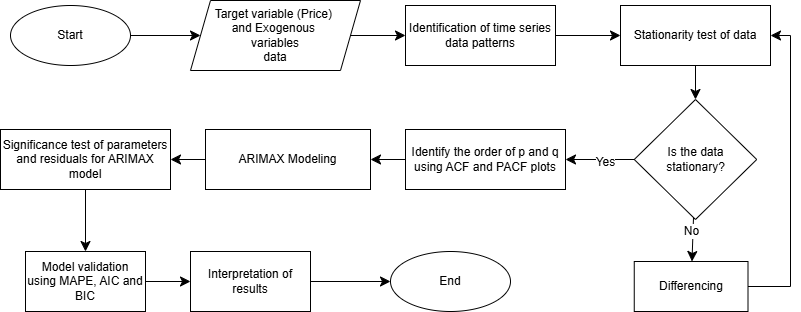
\includegraphics[width=\textwidth]{flowchart.png}
\end{frame}

% Error Metrics Frame 1
\begin{frame}{Error Metrics}

\begin{itemize}
    \item \textbf{Mean Absolute Error (MAE)}: The average of the absolute differences between the predicted and actual values. It provides a measure of how close predictions are to the actual outcomes. 
    $$
        MAE = \frac{1}{n} \sum_{i=1}^{n} |y_{i} - \hat{y}_{i}|  
    $$
    

    \item \textbf{Mean Absolute Percentage Error (MAPE)}: The average of the absolute percentage errors between the predicted and actual values. It is useful for understanding the accuracy of the model in relative terms.

    $$
        MAPE = \frac{1}{n} \sum_{i=1}^{n} \left| \frac{y_{i} - \hat{y}_{i}}{y_{i}} \right| \times 100  
    $$
\end{itemize}
\end{frame}

% Error Metrics Frame 2
\begin{frame}{Error Metrics (cont.)}
\begin{itemize}
    \item \textbf{Root Mean Square Error (RMSE)}: The square root of the average of the squared differences between predicted and actual values. It gives more weight to larger errors and is sensitive to outliers.
    
    $$
        RMSE = \sqrt{\frac{1}{n} \sum_{i=1}^{n} (y_{i} - \hat{y}_{i})^{2}}  
    $$
\end{itemize} 

Among these, MAPE is prioritized as the primary evaluation metric because of its interpretability in comparing the forecast accuracy. 
\end{frame}

% % Error Metrics Frame 3
\begin{frame}{MAPE Forecast Accuracy Rating}
\begin{table}
    \caption{\textit{MAPE Forecast Accuracy Rating}}
    \label{lewis}
    \centering
    \begin{tabular}{lc}
        \toprule
        MAPE (\%) & Forecast Accuracy \\
        \midrule
        $< 10\%$ & Highly accurate forecast \\
        $10\%$ to $<20\%$ & Good forecast \\
        $20\%$ to $< 50\%$ & Reasonable forecast \\
        $\ge 50\%$ & Inaccurate forecast \\
        \bottomrule
    \end{tabular}
\end{table}
\end{frame}

% Results and Discussion Introduction
\begin{frame}
    \begin{tcolorbox}[colframe=theme, colback=theme]
        \begin{center}
            \Huge{Results and Discussion}
        \end{center}
    \end{tcolorbox}
\end{frame}

\begin{frame}
    \begin{center}
        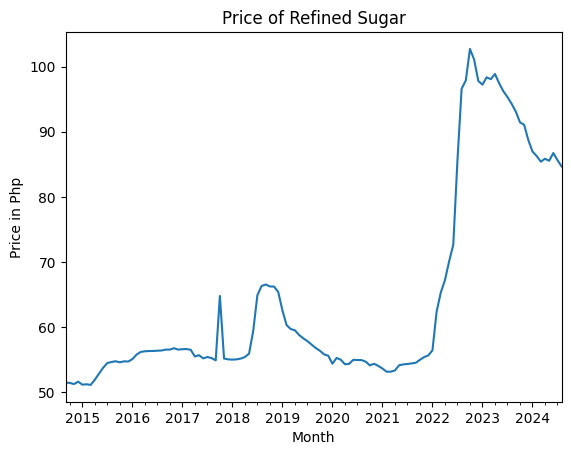
\includegraphics[width=0.75\textwidth, height =\textheight]{Price_plot.png}
    \end{center}
\end{frame}

\begin{frame}{Test for Stationarity}
    \begin{itemize}
        \item Performing the Augmented Dicky-Fuller test on the data shows a P-value of 0.664. 
        \item Performing first-order differencing results in p-value of 0.0000057. 
        \begin{center}
            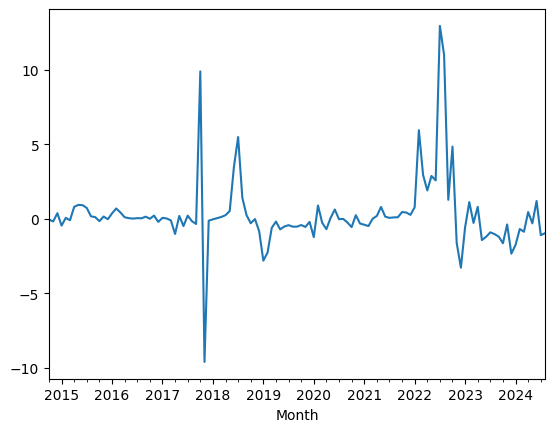
\includegraphics[width = 0.75\textwidth,height = .7\textheight]{differenced.png}
        \end{center}
    \end{itemize}
\end{frame}

\begin{frame}{Train-Test split}
    \begin{center}
        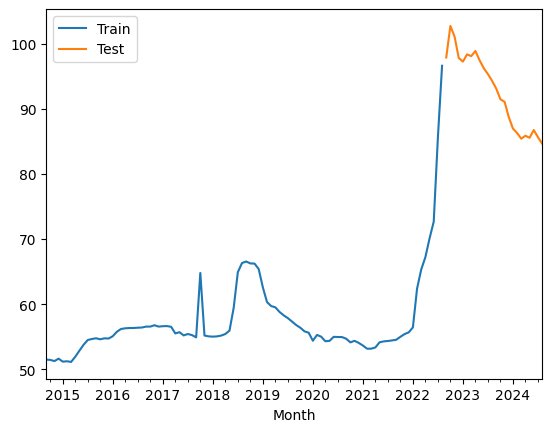
\includegraphics[width = 0.75\textwidth,height = .75\textheight]{split.png}
    \end{center}
\end{frame}

\begin{frame}{Order of $p$ and $q$}
        \begin{minipage}{0.48\textwidth}
        \centering
        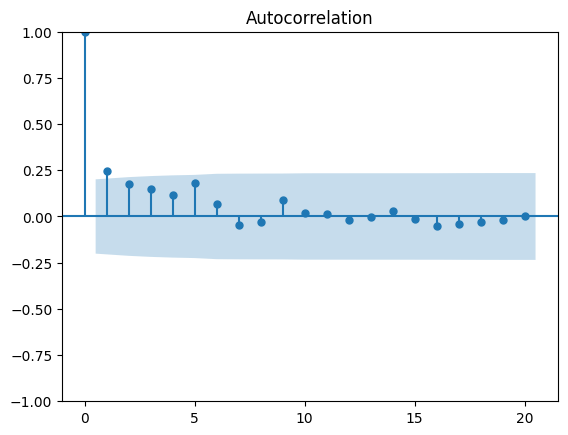
\includegraphics[width=\linewidth]{acf.png}
        $q = [1]$
    \end{minipage}
    \hfill
    \begin{minipage}{0.48\textwidth}
        \centering
        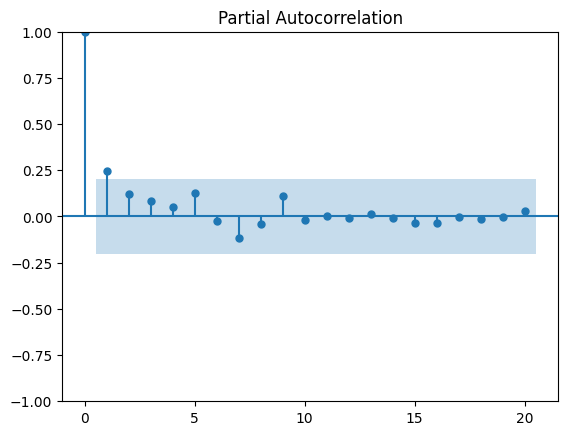
\includegraphics[width=\linewidth]{pacf.png}
            $p = [1]$ 
    \end{minipage}
\end{frame}

\begin{frame}{Selected Model}
        \begin{tcolorbox}[colframe=theme, colback=theme]
        \begin{center}
            \Huge{ARIMAX(1,1,1)}
        \end{center}
    \end{tcolorbox}
\end{frame}

\begin{frame}{Model evaluation}
    \begin{table}
    \caption{\textit{Performance Metrics of ARIMAX(1,1,1) Model}}
    \label{arimax111}
    \centering
    \begin{tabular}{lccccc}
        \toprule
        Model & MAE & MAPE & RMSE & AIC & BIC \\
        \midrule
        ARIMAX(1,1,1) & 4.58 & 5.21\% & 6.25 & 443.81 & 469.35 \\
        \bottomrule
    \end{tabular}
\end{table}
\end{frame}

\begin{frame}{Model evaluation}
    \begin{center}
        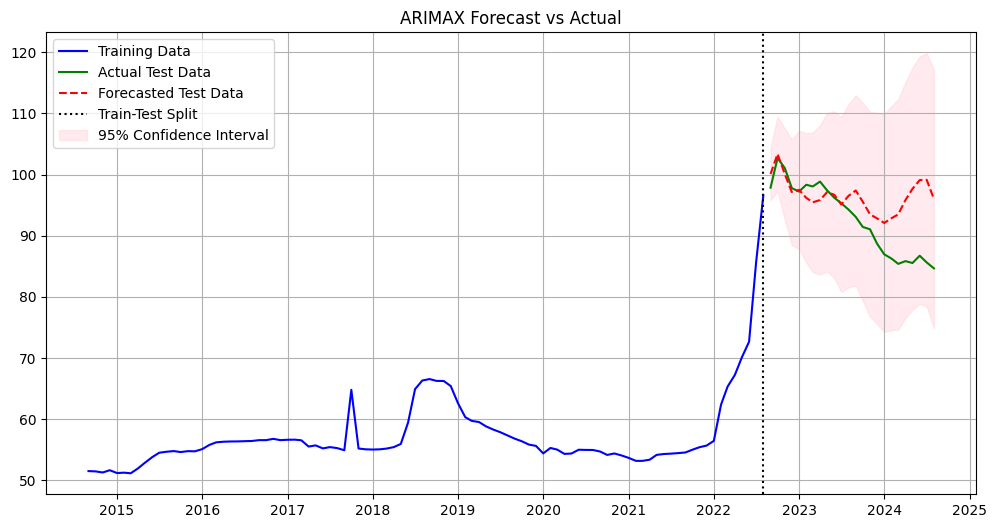
\includegraphics[width = .9\textwidth]{train_test_forecast.png}
    \end{center}
\end{frame}

\begin{frame}{Residual diagnostics}
    \begin{center}
         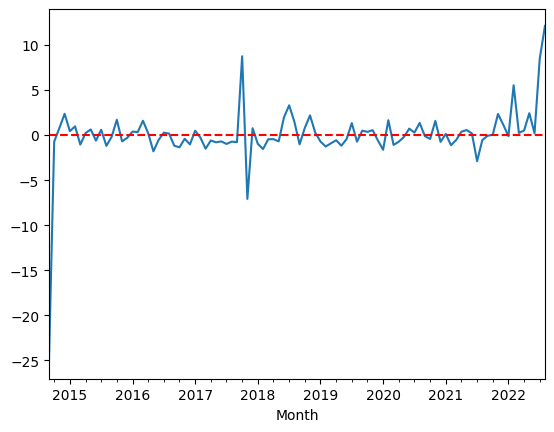
\includegraphics[width = 0.8\textwidth,height = .9\textheight]{resid.png}
    \end{center}
\end{frame}

\begin{frame}{Residual diagnostics}
    \begin{center}
           \begin{minipage}{0.48\textwidth}
        \centering
        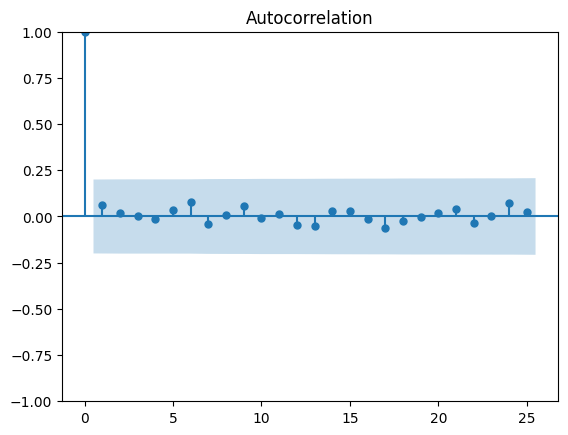
\includegraphics[width=\linewidth]{resid_acf.png}
    \end{minipage}
    \hfill
    \begin{minipage}{0.48\textwidth}
        \centering
        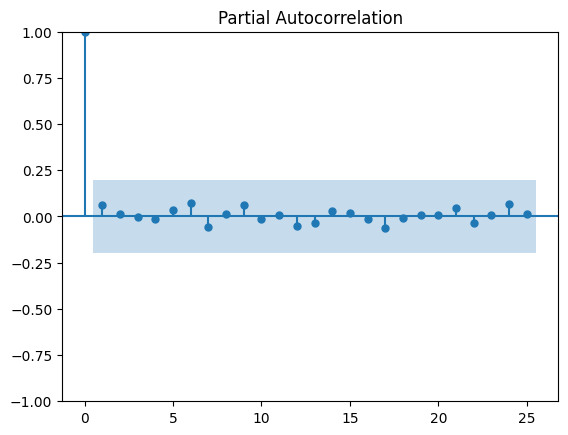
\includegraphics[width=\linewidth]{resid_pacf.png}
    \end{minipage}
    \end{center}
\end{frame}

\begin{frame}{Residual diagnostics}

    \textbf{Ljung-Box test}
    \begin{center}
                \begin{tabular}{cc|cc}
        \toprule
        Lag  & p-value & Lag & p-value  \\
        \midrule
        1  & 0.524 &  7 & 0.985 \\
        2  & 0.805 &  8 & 0.994 \\
        3  & 0.933 &  9 & 0.995 \\
        4  & 0.979 & 10 & 0.998 \\
        5  & 0.990 & 11 & 0.999 \\
        6  & 0.977 & 12 & 0.999 \\
        \bottomrule
    \end{tabular}
    \end{center}  

    The p-value for all 12 lags are higher than 0.05. Hence, the residuals shows no autocorrelation and it resembles white noise, increasing the validity of the model. 
\end{frame}

\begin{frame}{Test for Multicollinearity}
    \textbf{Variance Inflation Factor}
    \begin{center}
            \begin{tabular}{lc}
        \toprule
        Variable & VIF  \\
        \midrule
      Production  &  2.99 \\
      Withdrawals  &  1.77 \\
      Global Price  &  1.44     \\ 
      Exchange Rate  &   2.53    \\ 
      Temperature  &   1.2    \\ 
      Precipitation  &   2.56   \\
      Inflation &   2.23    \\ 
        \bottomrule
    \end{tabular}
    \end{center}
\end{frame}

\begin{frame}{ARIMAX(1,1,1) Model Summary}
    \begin{center}
            \begin{tabular}{lccr}
        \toprule
        Variable & Coefficient & P-value & Interpretation \\
        \midrule
        Production  & -2.006e-07 &  0.832  &  Not significant \\
        Withdrawals & 2.414e-07 &  0.811  &  Not significant  \\
       Global Price  & -10.4240   &  0.000  &  Highly significant \\ 
        Exchange Rate&  1.4639    &  0.000  &  Highly significant\\ 
        Temperature   &  0.2915    &  0.521  &  Not significant\\ 
        Precipitation &  0.0041    &  0.186  &  Somewhat significant \\
         Inflation &  0.8710    &  0.382  &  Not significant \\ 
        AR(1), MA(1)   &   ~0       & ~1.000  &  Not contributing to the model \\
        \bottomrule
    \end{tabular}
    \end{center}
\end{frame}

\begin{frame}{ARIMAX(1,1,1) Model Summary}
    The results of the summary shows that the following must be consider:
    \begin{enumerate}
        \item The coefficients for AR(1) and MA(1) are both zero and not contributing to the model. 
        \item Some of the variables are not significant based on their p-value, leaving Global Price and exchange rate with high significance.
        \item The coefficient of the Global Price is negative, which is counterintuitive.
    \end{enumerate}
\end{frame}

\begin{frame}{1. The coefficients for AR(1) and MA(1) are both zero and not contributing to the model}
      \begin{table}[H]
        \caption{\textit{Performance Metrics of ARIMAX(1,1,1) vs ARIMAX(0,1,0)}}
        \label{arimax010}
        \centering
        \begin{tabular}{lccccc}
            \toprule
            Model & MAE & MAPE & RMSE & AIC & BIC \\
            \midrule
            ARIMAX(1,1,1) & 4.58 & 5.21\% & 6.25 & 443.81 & 469.35 \\
            ARIMAX(0,1,0) & 4.58 & 5.21\% & 6.25 & 778.34 & 798.77 \\
            \bottomrule
        \end{tabular}
    \end{table}
\end{frame}

\begin{frame}{2. Some of the variables are not significant based on their p-value, leaving Global Price and exchange rate with high significance.}
    
      \begin{table}[H]
        \caption{\textit{Performance Metrics of ARIMAX(1,1,1) with all exogenous variable vs only the significant variables}}
        \label{exog_significant}
        \centering
        \begin{tabular}{lccccc}
            \toprule
            ARIMAX(1,1,1) & MAE & MAPE & RMSE & AIC & BIC \\
            \midrule
            With all Exogenous variables & 4.58 & 5.21\% & 6.25 & 443.81 & 469.35 \\
            Only the significant variables & 17.32 & 18.51\% & 17.72 & 668.23 & 688.66 \\
            \bottomrule
        \end{tabular}
    \end{table}
\end{frame}

\begin{frame}{3. The coefficient of the Global Price is negative, which is counterintuitive.}
           \begin{table}[H]
        \caption{\textit{Performance Metrics of ARIMAX(1,1,1) with global price vs no global price variable}}
        \label{noglobal}
        \centering
        \begin{tabular}{lccccc}
            \toprule
            ARIMAX(1,1,1) & MAE & MAPE & RMSE & AIC & BIC \\
            \midrule
            With global price & 4.58 & 5.21\% & 6.25 & 443.81 & 469.35 \\
            No global price  & 4.95 & 5.62\% & 6.60 & 442.03 & 465.02 \\
            \bottomrule
        \end{tabular}
    \end{table}
\end{frame}

% Evaluation
\begin{frame}{Key Takeaways from Modeling process}
  \begin{itemize}
    \item Residuals resemble white noise (Ljung-Box Test)
    \item No multicollinearity (checked via VIF)
    \item Global price variable excluded to improve interpretability
  \end{itemize}
\end{frame}

\begin{frame}
            \begin{tcolorbox}[colframe=theme, colback=theme]
        \begin{center}
            \Huge{Forecasting}
        \end{center}
    \end{tcolorbox}
\end{frame}

\begin{frame}{Forecasting the Price of Refined sugar for 2025 to 2027}
    \begin{center}
        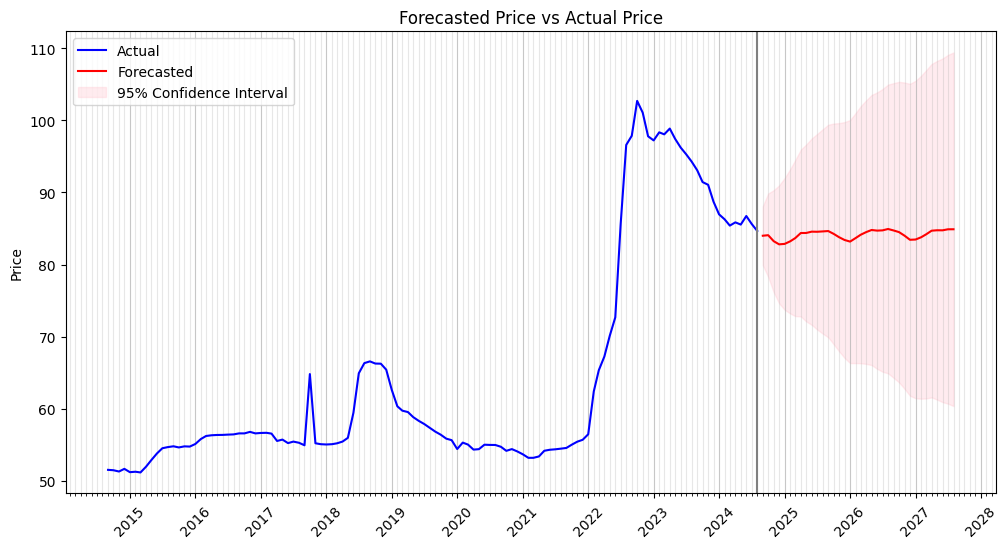
\includegraphics[width = 0.88\textwidth]{forecasted_plot.png}
    \end{center}
\end{frame}

\begin{frame}{Forecast Result Interpretation}
\begin{itemize}
    \item The 3-year forecast shows a relatively stable trend with mild fluctuations and a slight upward tendency over time. 
    \item The model is 95 percent confident that the actual price will lie within the confidence interval. 
    \item The forecasted price of refined sugar was ranging from 82.80 to 84.93 pesos per kilogram.
\end{itemize}
\end{frame}

\begin{frame}{Forecasted Prices vs the Latest Actual Prices}

     Retrieved from Department of Agriculture price monitoring (\textit{Bantay Presyo})

    \begin{table}[H]
    \label{super}
    \centering
    \begin{tabular}{lcc}
        \toprule
        Date & Actual Price & Forecasted Price  \\
        \midrule
        September 2024 & 84 &    83.99 \\
        October 2024   & 83.15 & 84.07  \\
        November 2024  & 83.13 & 83.23  \\
        December 2024  & 82.83 & 82.80  \\
        January 2025   & 83.65 & 82.86  \\
        February 2025  & 83.07 & 83.22  \\
        March 2025     & 83.14 & 83.67  \\
        April 2025     & 83.49 & 83.37  \\
        \bottomrule
    \end{tabular} 
\end{table}
\end{frame}


\begin{frame}{Forecasted Prices vs the Latest Actual Prices}

\begin{table}[H]
    \caption{\textit{Evaluation of the Forecasted price}}
    \label{eval}
    \centering
    \begin{tabular}{ccc}
        \toprule
         MAE & MAPE & RMSE \\
        \midrule
        0.43 & 0.51\% & 0.56 \\
        \bottomrule
    \end{tabular}
\end{table}
\end{frame}

\begin{frame}{Conclusion}
    
% Conclusion
\begin{itemize}
    \item Developed an ARIMAX(1,1,1) model to forecast monthly retail prices of refined sugar in the Philippines. 
    \item Integrated key exogenous variables: production, withdrawals, exchange rate, regional temperature, precipitation, and inflation rate. 
    \item Achieved high predictive accuracy:
        \begin{itemize}
            \item MAPE: 5.62\% (test set), 0.51\% (short-term validation). 
            \item MAE: 0.43, RMSE: 0.56 (short-term validation). 
        \end{itemize}
    \item Global price and exchange rate were statistically significant, but excluding global price improved model performance. 
    \item ARIMAX(1,1,1) outperformed other variants with the lowest AIC and BIC. 
    \item Three-year forecast shows stable prices with mild fluctuations and a slight upward trend (82.80 to 84.93 pesos/kg). 
\end{itemize}
\end{frame}

\begin{frame}{Recommendations}
\begin{itemize}
    \item \textbf{Larger datasets:} Use longer historical data (e.g., 20 years) and include additional exogenous variables like transportation costs, energy prices, and labor rates. 
    \item \textbf{Alternative models:} Explore models like SARIMAX, VARMA, VARMAX, or machine learning approaches (e.g., Random Forest, XGBoost, LSTM) for better performance. 
    \item \textbf{Statistical interpretation:} Investigate counterintuitive results, such as the negative coefficient for global sugar prices, to improve understanding.
\end{itemize}
\end{frame}

\begin{frame}
    \begin{tcolorbox}[colframe=theme, colback=theme]
        \begin{center}
            \Huge{Questions?}
        \end{center}
    \end{tcolorbox}
\end{frame}

\end{document}
